\documentclass[a4paper,10pt]{scrartcl}
\usepackage{fancyhdr}
\usepackage[utf8]{inputenc}
\usepackage[ngerman]{babel}
\usepackage{enumerate}
\usepackage[top=2cm, left=2cm, bottom=2cm, right=2cm]{geometry}
\usepackage{graphicx}
\usepackage{listings}
\usepackage{amsmath}
\usepackage{amsfonts}
\usepackage{amssymb}
\usepackage{float}

\pagestyle{fancy}
\fancyhf{}
\fancyhead[L]{\begin{small}Computer Graphics 2\\Übungsblatt 1\\Gruppe 5\end{small}}
\fancyhead[R]{\begin{small}Stürmer, Felix - 230127 - Informatik(Diplom) - stuermer@cs.tu-berlin.de\\
  Oskamp, Robert - 306952 - Mathematik(Diplom) - robert.oskamp@gmx.de\\
  Olthoff, Inken - 305844 - Mathematik(Diplom) - some-body@gmx.de\\
  Neumann, Cedrik - 301635 - Mathematik(Diplom) - c.neumann@live.de\end{small}}
\renewcommand{\headrulewidth}{0.4pt}
\fancyfoot[R]{\thepage}
\renewcommand{\footrulewidth}{0.4pt}


\begin{document}
\vspace*{1cm}
\begin{enumerate}[1.]

\item Der Algorithmus zum Auffinden des Medians in linearer Zeit sieht folgenderma"sen aus:\\
Sei $A$ eine Liste von Zahlen mit $|A| = n$, von denen wir den Median suchen und $k = \lfloor \frac{n}{2} \rfloor$ die Stelle an der wir den Median in einer sortierten Liste finden w"urden.\\
 Wenn $A$ weniger als z.B. $10$ Elemente besitzt, dann sortieren wir $A$ und geben das $k$-te Element aus.\\
 Ansonsten teilen wir $A$ in $\lceil \frac{n}{5} \rceil$ viele Teilmengen $S_i$, die aus (maximal) $5$ Elementen bestehen und suchen f"ur alle Teilmengen einzeln den Median $M_i$.\\
 Als n"achstes berechnen wir den Median $M$ der Mediane $M_i$ und teilen die Menge $A$ in drei disjunkte Teilmengen $A_1$, $A_2$ und $A_3$. Hierbei gilt f"ur die Mengen $a_1 < M ~\forall{a_1 \in A_1}$, $a_2 = M ~\forall{a_2 \in A_2}$ und $a_3 > M ~\forall{a_3 \in A_3}$.\\
Wenn jetzt f"ur $k$ gilt $k \leq |A_1|$, dann suche den Median in $A_1$ mit $k = k$.\\
Wenn f"ur $k$ gilt $k > |A_1| + |A_2|$, dann suche Median in $A_3$ mit $k = k - |A_1| - |A_2|$.\\
Wenn keine der beiden Bedingungen gilt, dann gib $M$ als Median aus.\\
\newline
Formal kann man auch schreiben:\\
\newline
median$(A,k)$ \{\\
    \hspace*{5 mm} if $(n \leq 10)$ \{\\
    \hspace*{10 mm} sort $A$\\
    \hspace*{10 mm} return the element at the $k$-th position of $A$\\
    \hspace*{5 mm} \}\\
    \hspace*{5 mm} partition $A$ into subsets $S_i$ of five elements\\
    \hspace*{5 mm} for $(i = 1, ~\dots ,~ n/5)$ \{\\
    \hspace*{10 mm} $M_i = $median$(S_i,3)$\\
    \hspace*{5 mm}\}\\
    \hspace*{5 mm} $M = $median$(\{M_i\}_{i=1,\dots,~ n/5},~ n/10)$\\
    \hspace*{5 mm} partition $A$ into $A_1$ with $a_1 < M ~\forall{a_1 \in A_1}$, $A_2$ with $a_2 = M ~\forall{a_2 \in A_2}$ and $A_3$ with $A_3 = A \setminus (A_1 \cup A_2)$\\
    \hspace*{5 mm} if $(k \leq |A_1|)$ \{\\
    \hspace*{10 mm} return median$(A_1,k)$\\
    \hspace*{5 mm} \}\\
    \hspace*{5 mm} else if $(k > |A_1| + |A_2|)$ \{\\
    \hspace*{10 mm} return median$(A_3, k - |A_1| - |A_2|)$\\
    \hspace*{5 mm} \}\\
    \hspace*{5 mm} else return $M$\\
    \}\\
\newline
F"ur die Laufzeit gilt:\\
$\begin{array}{r c l}\\
T(n)& \leq & \frac{12\cdot n}{5} + T(\frac{n}{5}) + T(\frac{7\cdot n}{10})\\
& = & \frac{12\cdot n}{5} + \frac{c\cdot n}{5} + \frac{7\cdot c\cdot n}{10}\\
& = & n\cdot (\frac{12}{5} + \frac{9\cdot c}{10})\\
\end{array}$\\
und damit ist die Laufzeit (asymptotisch) linear in $n$.

\item Sei $s$ die Kantenl"ange der kubischen Zelle und der Abstand der $n$ Punkte $\geq \varepsilon$.\\
In jedem Schritt halbieren wir die Kantenl"angen. Also haben im $k$-ten Schritt die kubischen Zellen die Kantenl"ange $s \cdot 2^{-k}$\\
Damit die $n$ Punkte sicher in verschiedenen kubischen Zellen liegen, muss die Diagonale der Zellen $< \varepsilon$ sein.\\
Somit erhalten wir eine maximale Tiefe $k$ f"ur die gilt:
$$s \cdot 2^{-k} < \frac{\varepsilon}{\sqrt{3}}$$
$$\Leftrightarrow k > -\log_2{\left( \frac{\varepsilon}{\sqrt{3}\cdot s}\right)} $$

\item
Betrachte ein Prisma, welches als Grundfläche ein gleichseitiges Dreick hat. Die Grundfläche ist so durch vier teilbar, dass wieder gleichseitige Dreiecke entstehen (siehe nachfolgende Skizze). Teilt man dann noch die Höhe des Prismas durch zwei, so erhält man aus einer solchen Prisma Zelle 8 translierte und um den Faktor 0.5 skalierte Prisma Zellen. Mit diesen Zellen kann jeweils wieder in gleicher Weise verfahren werden, so dass bei dieser Unterteilungsstrategie beliebig viele affin transformierte Versionen des Ausgangsprismas entstehen können.\\
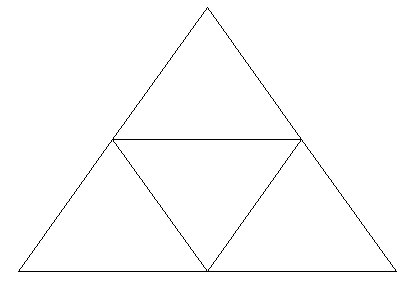
\includegraphics[scale=0.3]{triangle.png}

\item
Die Basisfunktionen f"ur einen B-Spline erster Ordnung sehen folgenderma"sen aus:\\
$N_i^1 (t) = \frac{t - t_i}{t_{i+1} - t_i} \cdot N_i^{0} (t) + \frac{t_{i+2} - t}{t_{i+2} - t_{i+1}} \cdot N_{i+1}^{0} (t)$\\
\newline
$N_i^1 (t) = \left\{
\begin{array}{ c l }
\frac{t - t_i}{t_{i+1} - t_i} \cdot N_i^{0} (t) &$ , falls $t_i \leq t < t_{i+1} \\
\frac{t_{i+2} - t}{t_{i+2} - t_{i+1}} \cdot N_{i+1}^{0} (t)  &$ , falls $t_{i+1} \leq t < t_{i+2} \\
0  &$ , sonst$ \\
\end{array} 
\right.$ \\
Ein B-Spline erster Ordnung für die Kontrollpunkte $d_0 = (0,0)$, $d_1 = (1,3)$, $d_2 = (2,1)$, $d_3 = (3,2)$ und $d_4 = (4,1)$ sieht wie folgt aus:\\
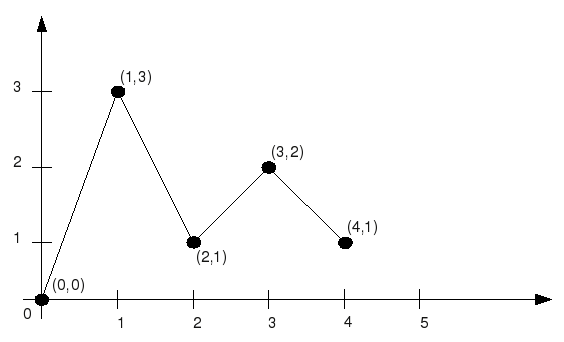
\includegraphics[scale=0.5]{spline.png}\\
Erklären Sie den Zusammenhang zwischen Grad, Stetigkeit und Träger bei B-Splines an diesem Beispiel.
Ein B-Spline vom Grad $g$ ist $g-1$ mal stetig differenzierbar, also in $C^{g-1}$, zusätzlich vergrößert sich mit höherem Grad der Träger. Im Beispiel haben Grad $g=1$ und sehen an den Kontrollpunkten Ecken, was darauf hindeutet, dass zwar Stetigkeit vorliegt, aber dass die Ableitung nicht mehr stetig ist, es liegt also $C^0$ Stetigkeit vor.

\item
Wir haben eine Kurve durch Kontrollpunkte $p_i$ im Raum gegeben, sowie Basisfunktionen $\beta_i(x)$.\\
Die Kontrollpunkte $p_i$ werden nun durch die Basisfunktionen $\beta_i$ gewichtet und addiert, so dass wir folgendes erhalten:
$$\sum_i{p_i \beta_i(x)}$$
F"ur diese so konstruierte Kurve soll nun affine Invarianz gilt, also
$$T \left( \sum_i{p_i \beta_i(x)}\right) = \sum_i{T p_i \beta_i(x)}$$
Dies gilt trivialerweise f"ur lineare Abbildungen.\\
Wir k"onnen unsere Transformation $T$ als linearen Abbildung mit einer Translation $T = A + a$ darstellen, wobei $A$ die lineare Abbildung und $a$ die Translation darstellt. (Wissen aus CG1)\\
Nun gilt f"ur unser T:
$$T \left( \sum_i{p_i \beta_i(x)}\right) = \sum_i{T p_i \beta_i(x)}$$
$$\Leftrightarrow \left( A + a \right) \left( \sum_i{p_i \beta_i(x)}\right) = \sum_i{\left( A + a \right) p_i \beta_i(x)}$$
$$\Leftrightarrow A\left( \sum_i{p_i \beta_i(x)}\right) + a = \sum_i{\left( A p_i \beta_i(x) + a \beta_i(x) \right)} $$
$$\Leftrightarrow A\left( \sum_i{p_i \beta_i(x)}\right) + a = \sum_i{A p_i \beta_i(x)} + \sum_i{a \beta_i(x)}$$
und dies gilt genau dann, wenn die $\beta_i$ an jeder Stelle eine Partition der Eins sind, also $\sum_i{\beta_i(x)} = 1 ~ \forall x$.\\

\end{enumerate}
\end{document}